% -*- root: main.tex -*-

\chapter{Apache Cassandra}
\label{chap:apache_cassandra}

Apache Cassandra jest bazą danych NoSQL\footnote{NoSQL (ang. Not Only SQL) - podzbiór baz danych, które zapewniają inne sposoby modelowania dziedziny niż tradycyjny model oparty na tabelach i~relacjach.}, która powstała w~wyniku połączenia rozwiązań wykorzystywanych w~Dynamo\footnote{Amazon DynamoDB - zdecentralizowana, wysoce skalowalna baza typu klucz-wartość.} oraz BigTable\footnote{Google BigTable - rozproszony system bazodanowy, który dobrze skaluje się dla ogromnych ilości danych.}. Cassandra początkowo była rozwijana dla potrzeb portalu społecznościowego Facebook. Baza danych powstała z~myślą o~rozwiązaniu problemu pełnotekstowego przeszukiwania skrzynek odbiorczych użytkowników, w~których dziennie zapisywane były miliardy wiadomości. Głównym celem, do którego dążyli twórcy Cassandry, była możliwość wykorzystania jej do przechowywania ogromnych ilości danych w~bardzo rozproszonym środowisku, gdzie awarie pojedynczych węzłów zdarzają się na porządku dziennym. W~tych warunkach baza danych musi zapewniać szybki i~niezawodny dostęp do danych. \cite{cassandra_introduction} 

Apache Cassandra wykorzystywana jest w~wielu serwisach na całym świecie. Najbardziej znaczące przykłady użycia produkcyjnego to eBay, Instagram oraz Github\footnote{eBay, Instagram, Github - przykłady dużych portali internetowych. eBay to serwis aukcyjny, Instagram to portal społecznościowy oparty o~publikację zdjęć wykonanych telefonami komórkowymi, a~Github to usługa pozwalająca na przechowywanie i~wersjonowanie kodu źródłowego aplikacji.}. Największa światowa instalacja Cassandry obejmuje około 15000 węzłów, na których przechowywane jest łącznie ponad 4 petabajty danych. \cite{official_cassandra}

W~przeciwieństwie do relacyjnych baz danych, Apache Cassandra nie zapewnia wsparcia dla reguły ACID\footnote{ACID (ang. Atomic, Consistency, Isolation, Durability) - zasada atomowości, spójności, izolacji i~trwałości. Wymienione cechy gwarantują poprawne przetwarzanie transakcji w~bazach danych.}. Zamiast tego zostały zrealizowane postulaty twierdzenia CAP: ,,we współdzielonym systemie plików można zachować maksymalnie dwie z~trzech właściwości: spójności, dostępności oraz podatności na partycjonowanie''. \cite{cap_theorem} Apache Cassandra priorytetyzuje właściwości dostępności oraz partycjonowania. Spójność danych jest odwrotnie proporcjonalna i~może być regulowana w~zależności od czasu odpowiedzi. Wysoka spójność danych oznacza wolniejszą odpowiedź bazy.

\section{Model danych}
\label{sec:cassandra_data_model}

Model danych Apache Cassandra jest analogiczny do BigTable. \cite{official_bigtable} Można przedstawić go jako dwuwymiarowa mapa trójek wartości:

\begin{figure}[ht!]
	\centering
	\verb+Map<RowKey, Map<ColumnKey, Triple<Value, Timestamp, TTL>>>+
\end{figure}

gdzie \verb+RowKey+ to identyfikator wiersza, \verb+ColumnKey+ to identyfikator kolumny, \verb+Value+ to wartość komórki, \verb+Timestamp+ to czas aktualizacji komórki, a~\verb+TTL+ to czas życia danej wartości. \cite{mc_fadin_long_live_data_model} Na rysunku \ref{fig:data_model_example} przedstawiona jest schematyczna ilustracja wiersza danych. Pogrubiona wartość w~lewej komórce to klucz wiersza, natomiast wyróżnione nagłówki oznaczają klucze poszczególnych kolumn. Każda komórka składa się z~trzech elementów: wartości, czasu życia oraz ,,odcisku czasu''.

\begin{figure}[ht!]
	\centering
	\begin{tabular}{|l||c|c|c|c|}
		\hhline{|-||----|}
		& \textbf{ABC} & \textbf{DEF} & $\cdots$ & \textbf{XYZ} \\
		\hhline{|~||====|}
		\textbf{123} & test value & another test value & $\cdots$ & not a~test value \\
		\cline{2-5}
		\textbf{456} & $20$ & $\infty$ & $\cdots$ & $\infty$ \\
		\cline{2-5}
		& 1291987837942000 & 1291980736812000 & $\cdots$ & 1291980736212000 \\
		\hhline{|-||----|}
	\end{tabular}

	\caption{Przykładowy wiersz modelu danych o~identyfikatorze 123456. Wartość komórki (123456, DEF) to ,,another test value''.}
	\label{fig:data_model_example}
\end{figure}

\section{Dystrybucja danych}
\label{sec:cassandra_data_distribution}

Do dystrybucji danych wykorzystywana jest funkcja skrótu, która zachowuje kolejność elementów. Węzły są rozmieszczone w~topologii pierścienia. Algorytm dystrybucji zostanie omówiony na przykładzie ze schematu~\ref{fig:data_distribution}: 

\begin{enumerate}
	\item Każdemu z~węzłów $\{A, B, C, D, E, F\}$ przypisywany jest token, który zawiera się w~zakresie wartości przyjmowanych przez funkcję skrótu. Strategię wyboru tokena można konfigurować. Przykładową strategią jest wybór losowy. W~omawianym przykładzie węzłom zostały przypisane tokeny o~wartościach $\{-16, -9, -3, 4, 9, 17\}$.
	\item Użytkownik bazy danych przesyła żądanie do dowolnego węzła, który pełni funkcję koordynatora dla danej operacji. Koordynator nadzoruje wpisanie danych do odpowiednich węzłów. W~omawianym przykładzie rolę koordynatora pełni węzeł~$E$.
	\item \label{en:master_node} Każdy węzeł przechowuje dane, których funkcja skrótu zawiera się w~przedziale $(token_{n-1}, token_{n}]$, gdzie $n$ to numer kolejny węzła rosnący zgodnie z~ruchem wskazówek zegara. W~przykładzie węzeł~$C$ przechowuje wiersze o~wartościach funkcji skrótu z~przedziału $(-9, -3]$, natomiast węzeł~$D$ z~przedziału $(-3, 4]$. Wartości funkcji obliczane są cyklicznie, stąd węzeł~$A$ przechowuje wiersze o~skrócie z~przedziału $(-\infty, -16] \cup (17, \infty)$. W~przykładzie wiersz o~kluczu z~funkcją skrótu wartości $-10$ zostanie utrwalony na węźle~$B$.
	\item Dane replikowane są na $n$ węzłach, gdzie $n$ to wartość konfigurowalnego współczynnika replikacji. Poza węzłem macierzystym (wyznaczanym w~punkcie \ref{en:master_node} algorytmu) dane są replikowane na $n - 1$ kolejnych (zgodnie z~ruchem wskazówek zegara) węzłach. W~omawianym przykładzie dane zostaną zreplikowane na węzłach~$C$~i~$D$.
\end{enumerate}

\begin{figure}[ht!]
	\centering
	
	\begin{tikzpicture}
		\def \n {6}
		\def \radius {3cm}
		\def \margin {10}

		\foreach \a/\b [count=\s] in {B/-9, A/-16, F/17, E/9, D/4, C/-3}
		{
  			\node[draw, circle, minimum width=1cm] at ({360/\n * (\s - 1)}:\radius) {$\a$};
  			\node at ({360/\n * (\s - 1)}:3.85cm) {$\b$};
  			\draw[>=latex] ({360/\n * (\s - 1)+\margin}:\radius) 
    			arc ({360/\n * (\s - 1)+\margin}:{360/\n * (\s)-\margin}:\radius);
		}

		\node[draw, rectangle, minimum height=1cm] at (-7.0, 0.0) {$data$};
		\draw[dashed, -triangle 45] (-6.95,0.5) arc (135:45:2.8cm);
		\node at (-5.1, 1.8) {$hash: -10$};
		\draw[-triangle 45] (-2.5, 0.0) arc (135:45:3.55cm);
		\draw[-triangle 45] (-2.5, 0.0) arc (90:32:4.5cm);
		\draw[-triangle 45] (-2.5, 0.0) arc (90:-30:1.45cm);
	\end{tikzpicture}

	\caption{Schematyczna ilustracja dystrybucji danych w~bazie danych Apache Cassandra.}
	\label{fig:data_distribution}
\end{figure}

\section{Algorytmy zapisu/usuwania danych}
\label{sec:data_storage_delete_algorithm}

Algorytm zapisu danych w~Apache Cassandra został schematycznie przedstawiony na diagramie~\ref{fig:cassandra_data_store_diagram}.~\cite{cassandra_write_internals} Składa się on z~następujących kroków:

\begin{figure}[ht!]
	\centering	
	\begin{tikzpicture}
		\node(stored-data)[draw, circle, text width=2cm, align=center] at (-2.0, 0.0) {Zapisywane dane};
		\node(memtable) [draw, rectangle, minimum width=2cm, minimum height=2cm] at (8.0, 0.0) {};
		\node[draw, rectangle, minimum width=0.5cm, minimum height=0.5cm] at (7.25, 0.75) {};
		\node[draw, rectangle, minimum width=0.5cm, minimum height=0.5cm] at (7.25, 0.25) {};
		\node[draw, rectangle, minimum width=0.5cm, minimum height=0.5cm] at (7.25, -0.25) {};
		\node[draw, rectangle, minimum width=0.5cm, minimum height=0.5cm] at (7.25, -0.75) {};
		\node[draw, rectangle, minimum width=0.5cm, minimum height=0.5cm] at (7.75, 0.75) {};
		\node[draw, rectangle, minimum width=0.5cm, minimum height=0.5cm] at (7.75, 0.25) {};
		\node[draw, rectangle, minimum width=0.5cm, minimum height=0.5cm] at (7.75, -0.25) {};
		\node[draw, rectangle, minimum width=0.5cm, minimum height=0.5cm] at (7.75, -0.75) {};
		\node[draw, rectangle, minimum width=0.5cm, minimum height=0.5cm] at (8.25, 0.75) {};
		\node[draw, rectangle, minimum width=0.5cm, minimum height=0.5cm] at (8.25, 0.25) {};
		\node[draw, rectangle, minimum width=0.5cm, minimum height=0.5cm] at (8.25, -0.25) {};
		\node[draw, rectangle, minimum width=0.5cm, minimum height=0.5cm] at (8.25, -0.75) {};
		\node[draw, rectangle, minimum width=0.5cm, minimum height=0.5cm] at (8.75, 0.75) {};
		\node[draw, rectangle, minimum width=0.5cm, minimum height=0.5cm] at (8.75, 0.25) {};
		\node[draw, rectangle, minimum width=0.5cm, minimum height=0.5cm] at (8.75, -0.25) {};
		\node[draw, rectangle, minimum width=0.5cm, minimum height=0.5cm] at (8.75, -0.75) {};
		\node[below of=memtable, yshift=-0.5cm] {$memtable$};
		\draw [-triangle 45] (stored-data) -- (memtable);
		\node(commitlog)[cylinder, draw, shape aspect=0.3, shape border rotate=90, minimum height=1cm] at (1.0, -5.0) {$commit$ $log$};
		\draw [-triangle 90] (1.0, 0.0) -- (commitlog);
		\node(sstable)[draw, rectangle, rounded corners, minimum height=2cm, minimum width=5cm] at (7.0, -4.5) {};
		\draw [-] (6.5, -5.5) -- (6.5, -3.5);
		\node[text width=2.5cm, align=center] at (8, -4.5) {$SSTable$};
		\node[text width=1cm, align=center] at (5.15, -4) {$INDEX$};
		\draw [-, dashed] (memtable) -- (10.0, 0.0);
		\draw [-, dashed] (10.0, 0.0) -- (10.0, -4.5);
		\draw [-triangle 45, dashed] (10.0, -4.5) -- (sstable);
		\draw[-, dashed, thick] (-3.25, -2.4) -- (10.25, -2.4);
		\node[align=center] at (-1.65, -2) {\footnotesize Pamięć operacyjna};
		\node[align=center] at (-2, -2.75) {\footnotesize Pamięć trwała};
	\end{tikzpicture}

	\caption{Schematyczna ilustracja algorytmu zapisu danych dla Cassandry.}
	\label{fig:cassandra_data_store_diagram}
\end{figure}

\begin{enumerate}
	\item Do węzła przesyłane są dane, które mają zostać na nim zapisane. 
	\item Dane kopiowane są do dwóch struktur:
		\begin{itemize}
			\item \emph{memtable} - przechowuje wiersze w~pamięci operacyjnej,
			\item \emph{commit log} - przechowuje informacje o~kolejnych zapisach wykonywanych do bazy danych.
		\end{itemize}
	\item Podstawową strukturą do pobierania danych jest \emph{memtable}. Jest ona umieszczona w~szybkiej pamięci, zapewnia więc krótki czas dostępu do danych. Wykorzystanie trwałej struktury \emph{commit log} pozwala na odtworzenie zawartości \emph{memtable} w~przypadku awarii wymagającej nagłego restartu maszyny, na przykład braku zasilania. Przy ponownym uruchomieniu węzła Cassandry odtwarza on kolejno wszystkie zapisy, które znajdują się w~\emph{commit logu}.
	\item W~przypadku przepełnienia \emph{memtable} wykonywane jest ,,spłukiwanie'' zawartości pamięci na dysk do struktury nazywanej \emph{SSTable}. Poza danymi zawiera ona indeks, który pozwala na szybki dostęp do danych wierszy. Jej charakterystyczną cechą jest niezmienność. Po przepisaniu danych z~\emph{memtable} do \emph{SSTable} jej zawartość nie jest już modyfikowana. Z~tego względu wiersze o~tym samym kluczu są często podzielone pomiędzy wiele takich struktur. ,,Spłukiwanie'' może zostać uruchomione manualnie z~wykorzystaniem polecenia \verb+nodetool flush+.
	\item Ostatnim etapem zapisu danych jest kompresja. Aktualizacja danych nie może nadpisywać istniejących wierszy, bo struktura \emph{SSTable} jest niezmienna. Zamiast tego wstawia ona rekordy z~późniejszym ,,odciskiem czasu''. Powoduje to nadmiarowe zużycie przestrzeni dyskowej. Kompresja pozwala usunąć nieaktualne wierwsze poprzez przepisanie istniejących \emph{SSTable} na nowe, uporządkowane struktury. Kompresja może być wywoływana automatycznie w~zależności od wybranej strategii lub manualnie, z~wykorzystaniem polecenia \verb+nodetool compact+.
\end{enumerate}

Niemodyfikowalność struktur \emph{SSTable} ma swoje konsekwencje także dla operacji usuwania danych. Wiersz nie może zostać fizycznie skasowany. Zamiast tego oznacza się go specjalnym znacznikiem \emph{tombstone}. Wiersze oznaczone tą flagą są usuwane na etapie kompresji danych.

\section{Obszary zastosowania Cassandry}
\label{sec:cassandra_usage_areas}

Specyficzny schemat danych Apache Cassandry i~brak wielu mechanizmów znanych z~relacyjnych systemów bazodanowych powodują, że nie jest ona najlepszym wyborem do przechowywania uniwersalnych danych:

\begin{itemize}
	\item Brak wsparcia dla transakcji znacząco utrudnia wykorzystanie Cassandry w~dziedzinach, dla których spójność danych jest kwestią kluczową. Przykładem może być obszar finansowy. W~systemach relacyjnych spójność jest zapewniona poprzez mechanizmy bazy danych. W~przypadku Apache Cassandry odpowiedzialność zostaje przeniesiona na aplikacje dostępowe, co znacząco zwiększa ilość pracy koncepcyjnej i~zwiększa ryzyko błędów.
	\item Brak możliwości złączania powoduje, że model danych musi być projektowany w~oparciu o~wykonywane do niego odwołania. Utrudnia to rozbudowę aplikacji. Przykładowo dla relacji jeden do wielu modelowanej poprzez tabelę, w~której identyfikatorem wiersza jest identyfikator obiektu nadrzędnego, a~w~kolumnach wpisywane są identyfikatory obiektów podrzędnych, nie jest możliwe zwrócenie wszystkich obiektów nadrzędnych wskazujących na dany obiekt podrzędny bez modyfikacji schematu.
	\item Brak złączeń implikuje denormalizację modelu danych. Wprowadza to problemy z~zachowaniem spójności. Aby zaktualizować adres, który jest przechowywany w~formie zdenormalizowanej w~tabeli użytkownika oraz zamówienia, należy znaleźć wszystkie rekordy, które wskazują na ten adres. Odpowiedzialność za spójność danych ponownie zostaje przeniesiona na aplikację, która wykorzystuje bazę.
\end{itemize}

W~tabeli~\ref{tab:cassanda_relationship_database_comparison} przedstawiono porównanie różnych aspektów Apache Cassandry i~relacyjnych systemów bazodanowych. Analizując informacje zebrane w~tabeli i~przedstawione wcześniej w~rozdziale można wyciągnąć następujące wnioski:

\begin{figure}[ht!]
	\begin{minipage}{\textwidth}
		\setcounter{mpfootnote}{6}
		\centering

		\begin{tabular}{|p{3cm}|p{4.5cm}|p{4.5cm}|}
			\hline
			& {\small \textbf{Apache Cassandra}} & {\small \textbf{RDBMS}} \\
			\hline
			{\small \textbf{Skalowalność horyzontalna}} &
			Liniowa skalowalność horyzontalna. &
			Pod warunkiem wykorzystania specjalnych narzędzi i/lub technik, na przykład \emph{shardingu}\footnotemark{}. \\
			\hline
			{\small \textbf{Mechanizmy zachowywania spójności}} &
			Brak mechanizmów zachowywania spójności danych. &
			Mechanizmy i~model zapewniające wysoką spójność danych. Wsparcie dla transakcyjności; znormalizowany model. \\
			\hline
			{\small \textbf{Odporność na awarie}} &
			Wysoka odporność na awarie zapewniona między innymi przez replikację danych pomiędzy węzłami. &
			Niska odporność na defekty. Pojedynczy punkt awarii. \\
			\hline
			{\small \textbf{Optymalizacja operacji}} &
			Optymalizacja pod kątem szybkości zapisu. &
			Optymalizacja pod kątem szybkości wykonywania zapytań. \\
			\hline
			{\small \textbf{Koncepcja}} &
			Projekt z~myślą o~opisywaniu szeregu chronologicznego danych.~\cite{why_should_i_use_cassandra} &
			Projekt do opisu uniwersalnych, ustrukturyzowanych danych. \\
			\hline
			{\small \textbf{Przystosowanie modelu danych}} &
			Model odpowiedni dla dynamicznych struktur danych zmieniających się w~trakcie działania systemu.~\cite{consider_cassandra} &
			Model odpowiedni dla niezmiennych struktur danych. \\
			\hline
		\end{tabular}

		\footnotetext{Sharding (od \emph{shard} - ang. kawałek) - technika polegająca na podziale zbioru danych na niezależne partycje w~zależności od ich cech, na przykład grupując użytkowników według lokalizacji geograficznej.~\cite{database_sharding}}

		\caption{Porównanie Apache Cassandry z~relacyjnymi bazami danych.}
		\label{tab:cassanda_relationship_database_comparison}
	\end{minipage}
\end{figure}

\begin{itemize}
	\item Modelowanie dziedziny danych jest znacznie prostsze w~przypadku systemów relacyjnych. Na etapie projektowania nie trzeba brać pod uwagę wykonywanych odwołań, potencjalnych problemów niespójności, a~także możliwych kierunków rozbudowy aplikacji.
	\item Apache Cassandra najlepiej sprawdza się w~zastosowaniu do \emph{big data}. Do poszczególnych fragmentów definicji wielkich zbiorów danych, która została przytoczona w~sekcji~\ref{sec:motivation}, można przyporządkować cechy charakteryzujące Cassandrę:
		\begin{itemize}
			\item ,,dużych rozmiarów'' - liniowa skalowalność horyzontalna pozwala na obsługę informacji o~dowolnej wielkości, pod warunkiem zapewnienia odpowiedniej liczby węzłów,
			\item ,,różnorodnych'' - model danych nie jest sztywny, może być dostosowany do zmieniających się danych w~trakcie działania aplikacji,
			\item ,,często zmieniających się'' - wbudowana obsługa szeregu chronologicznego oraz optymalizacja czasu zapisu zostały zaprojektowane pod kątem dynamicznie zmieniających się danych. 
		\end{itemize}
\end{itemize}

\noindent Według twórców Cassandry~\cite{why_migrate_from_mysql} typowymi obszarami jej zastosowań są:

\begin{itemize}
	\item Aplikacje wykonujące OLTP\footnote{On-Line Transaction Processing - przetwarzanie transakcji sieciowych.}, a~więc transakcje charakteryzujące się wysoką współbieżnością, krótkim czasem odpowiedzi, małymi zapytaniami oraz pracą na dużych zbiorach danych.~\cite{oltp_definition}
	\item Zarządzanie danymi uszeregowanymi w~czasie.
	\item Pobieranie i~analiza danych z~urządzeń o~wysokiej częstotliwości odświeżania informacji.
	\item Aplikacje typu SaaS\footnote{Software as a Service (ang. oprogramowanie jako usługa sieciowa) - aplikacje, które mogą być wykorzystywane przez sieć bez pobierania i~instalacji na stacji roboczej.~\cite{saas_definition} Przykładem takiej aplikacji jest Google Docs (\url{https://docs.google.com/}), który umożliwia edycję dokumentów, arkuszy kalkulacyjnych oraz prezentacji z~wykorzystaniem przeglądarki internetowej.} oparte o~intensywne wykorzystanie usług sieciowych.
	\item Zarządzanie mediami strumieniowymi (muzyka, filmy) oraz nieustrukturyzowanymi danymi (dobrym przykładem są portale społecznościowe).
	\item \textbf{Systemy ,,zapisochłonne''}.
\end{itemize}

Z~przedstawionych scenariuszy Autor zdecydował się wyróżnić ostatni. Istotnym zagadnieniem w~przypadku wielkich danych jest operacja zapisu, która musi być wykonywana w~czasie rzeczywistym. Aby omówić problem należy przedstawić typową architekturę wykorzystywaną w~relacyjnych bazach danych do przechowywania wielkich danych.~\cite{sharding_in_mysql} Prezentuje ją diagram~\ref{fig:sharding}.

\begin{figure}[ht!]
	\centering
	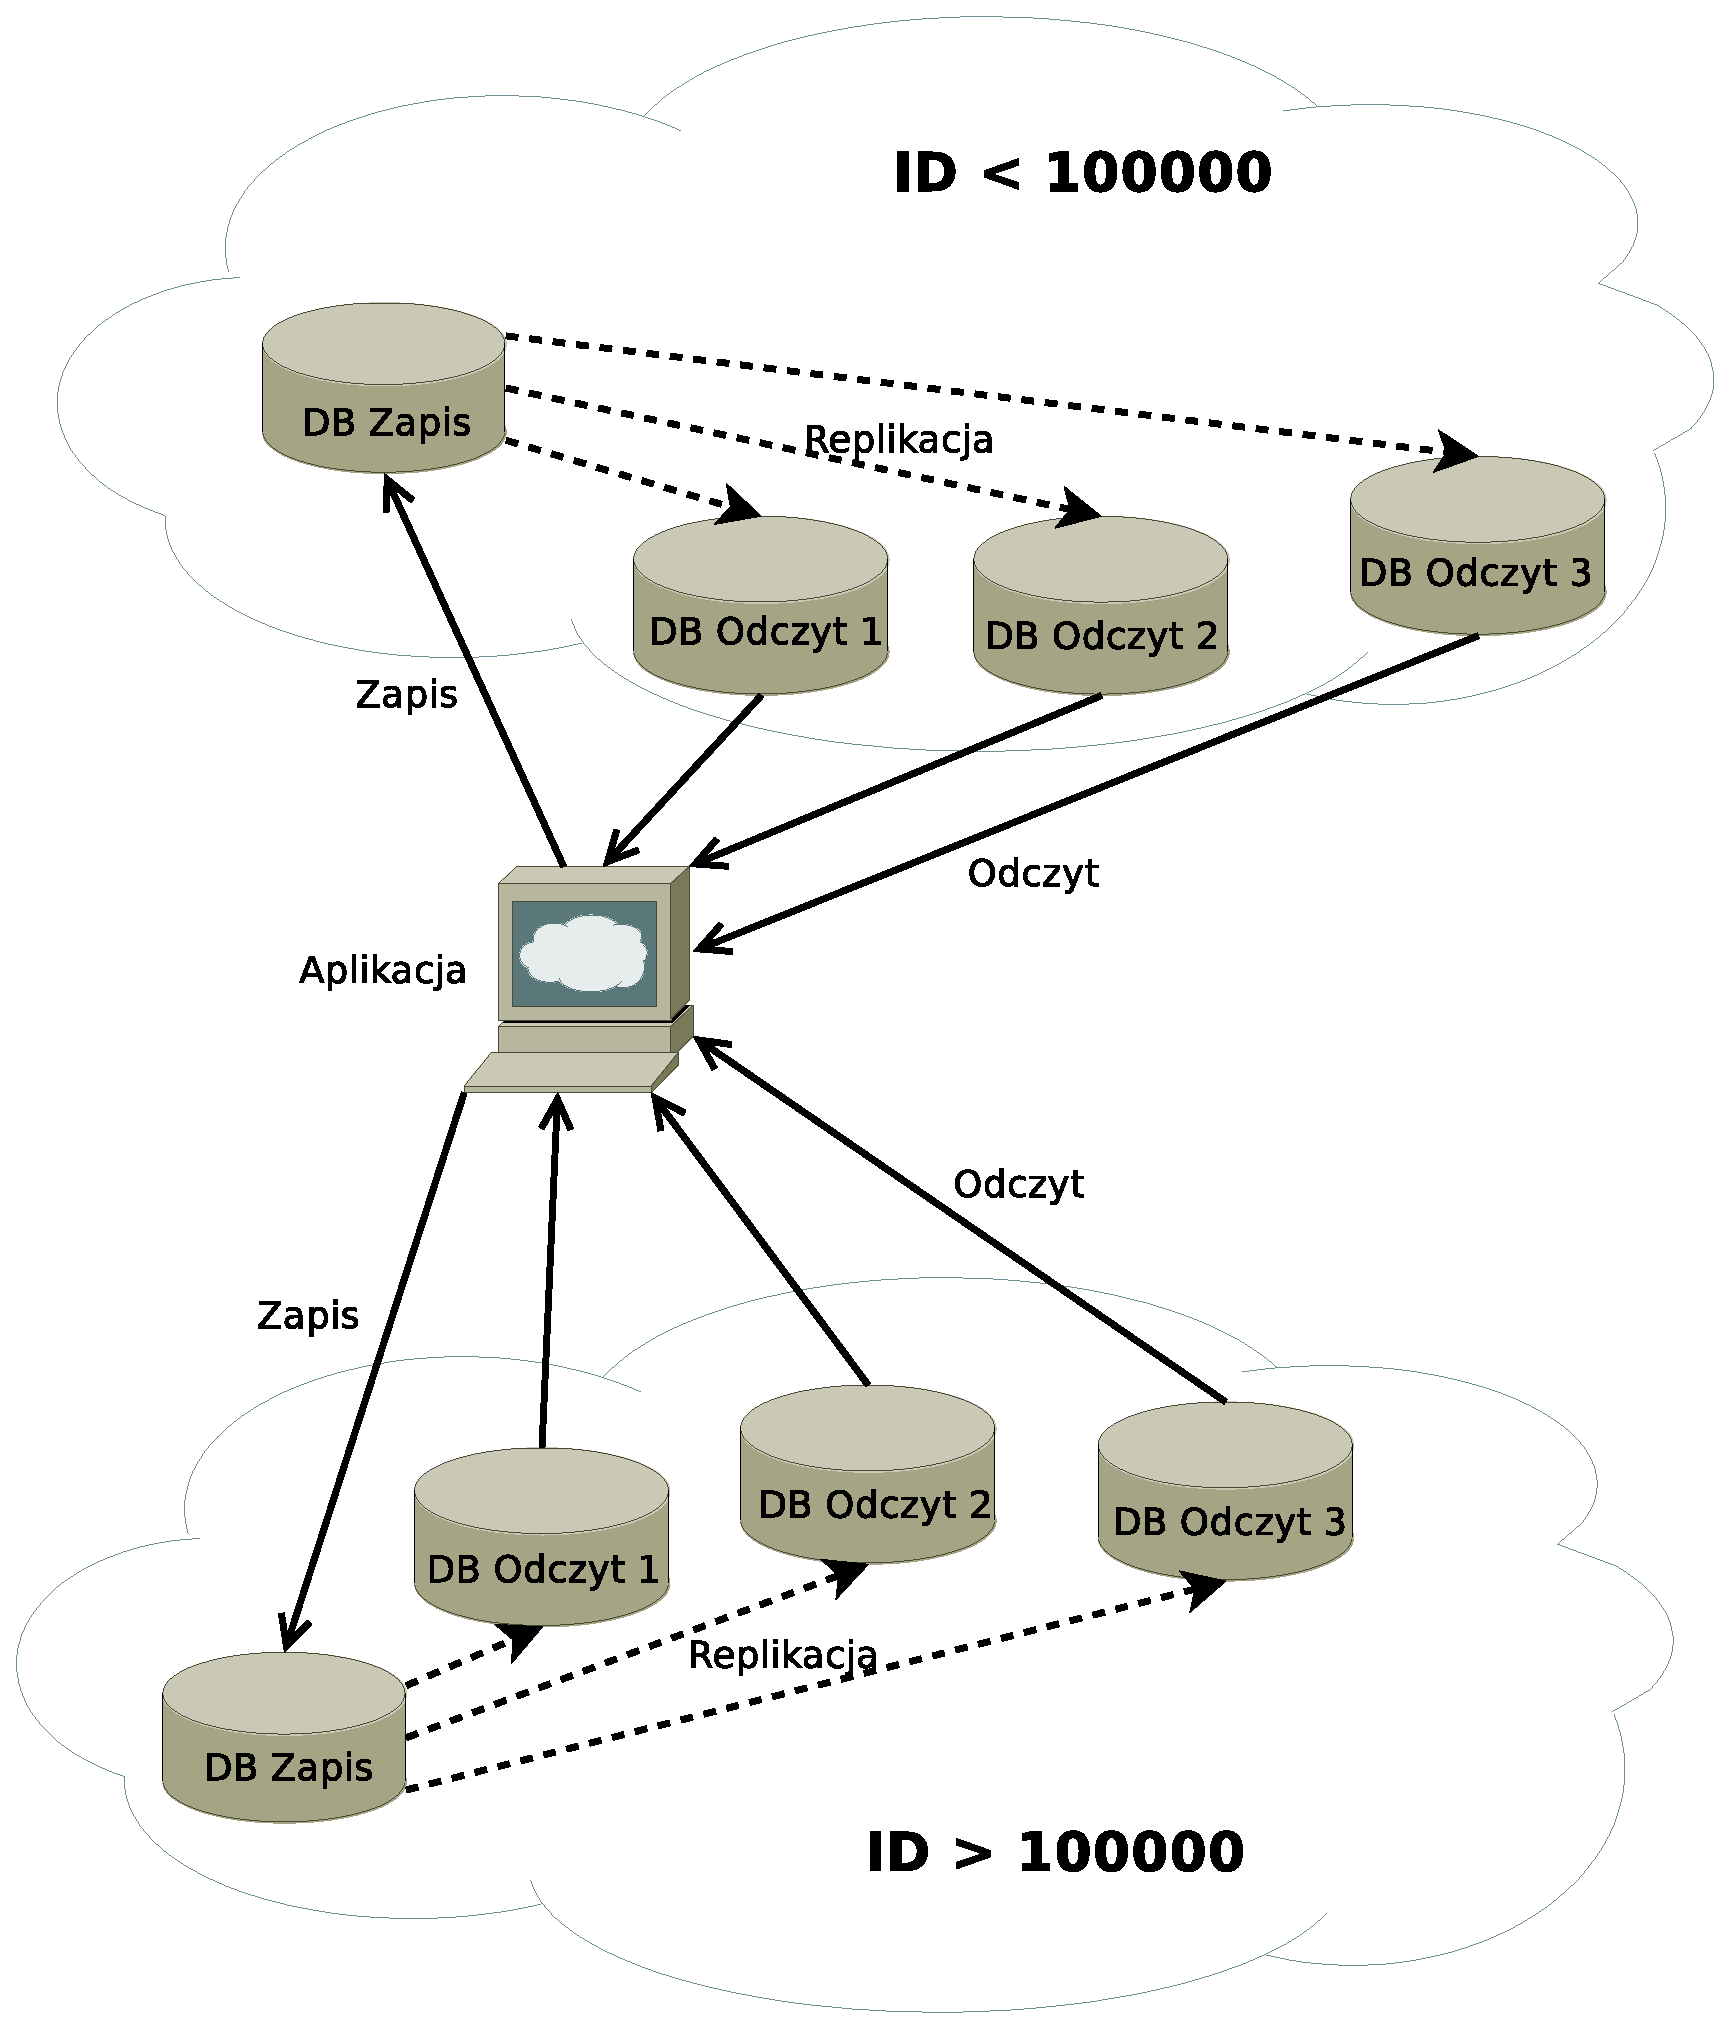
\includegraphics[width=.8\textwidth]{figures/sharding.eps}
	\caption{Schematyczna ilustracja partycjonowania relacyjnej bazy danych (określanego angielskim terminem \emph{sharding}).}
	\label{fig:sharding}
\end{figure}

Na diagramie przedstawiono aplikację, która odwołuje się do relacyjnej bazy danych. Została ona podzielona na dwie partycje względem identyfikatora wiersza (mniejszy lub większy od 100000). Każda partycja zawiera jeden węzeł, który wykonuje operacje zapisu (\verb+DB Zapis+). Do niego odwołuje się aplikacja z~żądaniem zapisu danych. W~każdej partycji znajdują się również trzy węzły, które pozwalają na odczyt danych (\verb+DB Odczyt+). Aplikacja zwraca się o~odczyt danych kolejno do różnych węzłów. Pozwala to zbalansować obciążenie. Należy zauważyć, że w~przedstawionej architekturze aplikacja musi wiedzieć, do której partycji należy się odwołać aby pobrać odpowiednie dane.

Proces skalowania systemu o~przedstawionej architekturze jest dwustopniowy:

\begin{enumerate}
	\item Skalowanie operacji odczytu. Może zostać przeprowadzone dla każdej partycji osobno. Polega na dodaniu nowego węzła, który służy do odczytu danych. Jest to stosunkowo proste, należy jednak uwzględnić dodany punkt dostępu w~puli serwerów, do których odwołuje się aplikacja.
	\item Skalowanie operacji zapisu. W~tym przypadku nie wystarczy dodanie drugiego węzła odpowiedzialnego za zapis, gdyż dane i~tak muszą zostać zreplikowane pomiędzy węzłami. Z~tego względu obciążenie obu serwerów pozostałoby bez zmian. Skalowanie operacji zapisu to skomplikowany proces wymagający stworzenia nowej partycji i~modyfikacji reguł przydzielania rekordów do poszczególnych fragmentów. 
\end{enumerate}

Podobna architektura wykorzystywana jest w~komercyjnych rozwiązaniach, takich jak \verb+MySQL Cluster CGE+\footnote{Strona domowa projektu - \url{http://www.mysql.com/products/cluster/}.}. Występują tam dodatkowe warstwy pośredniczące, które ukrywają szczegóły wykonywania zapytań przed aplikacją. Sama zasada działania pozostaje jednak analogiczna.

Problemem w~tej architekturze pozostaje skalowanie operacji zapisu. Może ono zostać wykonane poprawnie tylko pod warunkiem, że istnieje funkcja partycjonująca dla danego natężenia operacji zapisu, która dzieli całość danych na dostatecznie wydajne (a~więc małe) fragmenty. Okazuje się, że w~praktyce nie zawsze jest to możliwe. Właśnie ten problem przyczynił się do powstania projektu Apache Cassandra w~Facebooku. 

Wszystkie przypadki użycia wymienione przez twórców Cassandry pokrywają scenariusze, w~których ich system bazodanowy sprawdza się lepiej niż podejście relacyjne w~subiektywnym odczuciu. Omówiony szerzej przypadek z~zapisem jest jednak jedynym, który z~przyczyn technologicznych może być nierealizowalny w~świecie SQL-owych baz danych.

\section{Struktura danych a~modelowanie}
\label{sec:relative_vs_cassandra_model}

Struktura i~mechanizm dystrybucji danych wykorzystywany w~Apache Cassandrze zmieniają podejście do modelowania dziedziny znane z~relacyjnych baz danych. Zbudowanie efektywnego modelu danych Cassandry wymaga skupienia się w~podobnym stopniu na zdefiniowaniu encji z~modelowanego świata, jak również na analizie odwołań, które będą wykonywane do obiektów z~tego świata.~\cite{modeling_best_practices_pt_1}

Załóżmy, że celem jest modelowanie danych dla sklepu internetowego. Zakupów dokonują użytkownicy, którzy mogą wstawić wiele przedmiotów z~oferty sklepu na listę życzeń. W~przypadku baz opartych o~język SQL jest to klasyczny problem relacji typu wiele-do-wielu, do modelowania których wykorzystywana jest najczęściej tabela pośrednia. 

\begin{figure}[ht!]
	\centering
	\scalebox{0.85}{
		\begin{tikzpicture}
			\umlclass[x=-5.7, y=0]{User}
			{
				\umlstatic{userId : int} $<$PK$>$ \\
			}
			{
				name : varchar(255) \\
				surname : varchar(255) \\
			}

			\umlclass[x=0, y=0]{Wishlist}
			{
				\umlstatic{wishlistId : int} $<$PK$>$ \\
			}
			{
				userId : int $<$FK$>$ \\
				itemId: int $<$FK$>$ \\
			}

			\umlclass[x=5.5, y=0]{Item}
			{
				\umlstatic{itemId : int} $<$PK$>$
			}
			{
				name : varchar(255) \\
				price : number(10, 2) \\
				desc : varchar(1024) \\
				category : varchar(255) \\
				weight : number(10, 2) \\
			}
			\umluniassoc[mult1=1, mult2=*]{User}{Wishlist}
			\umluniassoc[mult1=1, mult2=*]{Item}{Wishlist}
			\node at (-2.8, 0.25) {\footnotesize wants};
			\node at (2.7, -0.25) {\footnotesize is on};
		\end{tikzpicture}
	}

	\caption{Modelowanie listy życzeń w~relacyjnej bazie danych.}
	\label{fig:er_wishlist}
\end{figure}

Diagram prezentujący zamodelowaną relację dla listy życzeń jest przedstawiony na rysunku~\ref{fig:er_wishlist}. W~tabeli Użytkownik (\emph{User}) przechowywane są imię, nazwisko oraz identyfikator. W~tabeli Przedmiot (\emph{Item}) znajduje się nazwa, cena, a~także inne właściwości: opis, kategoria oraz waga. Tabela Lista życzeń (\emph{Wishlist}) łączy ze sobą użytkownika i~przedmiot poprzez wykorzystanie kluczy obcych. 

Powyższy model jest wykorzystywany w~widoku listy życzeń na profilu użytkownika. Na liście życzeń prezentowane są informacje o~nazwie przedmiotu oraz jego cenie. Po kliknięciu nazwy użytkownik przenoszony jest do strony przedmiotu. Na listingu~\ref{lst:sql_wishlist} zaprezentowano zapytanie, które wyświetla listę życzeń.

\begin{verbbox}[\footnotesize]
	SELECT item.name, item.price
	FROM Item item, Wishlist wishlist
	WHERE wishlist.userId = 202;
\end{verbbox}

\begin{figure}[ht!]
	\centering
	\theverbbox

	\caption{Zapytanie, które pobiera wszystkie przedmioty na liście życzeń użytkownika o~identyfikatorze 202.}
	\label{lst:sql_wishlist}
\end{figure}

Cassandra umożliwia utworzenie dokładnej repliki relacyjnego modelu danych. Zostało to przedstawione na rysunku~\ref{tab:bad_cassandra_data_model}.

\begin{figure}[ht!]
	\centering

	\begin{tabular}{llll}
		User &
		\begin{tabular}{|l||c|c|}
			\hhline{|-||--|}
			& \textbf{name} & \textbf{surname} \\
			\hhline{|~||==|}
			\textbf{123} & Janusz & Kowalski \\
			\hhline{=::==}
			& \textbf{name} & \textbf{surname} \\
			\hhline{|~||==|}
			\textbf{124} & Marcin & Nowak \\
			\hhline{|-||--|}
		\end{tabular} &
		Wishlist & 
		\begin{tabular}{|l||c|c|}
			\hhline{|-||--|}
			& \textbf{userId} & \textbf{itemId} \\
			\hhline{|~||==|}
			\textbf{51} & 123 & 579 \\
			\hhline{=::==}
			& \textbf{userId} & \textbf{itemId} \\
			\hhline{|~||==|}
			\textbf{52} & 124 & 232 \\
			\hhline{|-||--|}
		\end{tabular} \\
	\end{tabular}

	\vspace{2em}

	\begin{tabular}{ll}
		Item &
		\begin{tabular}{|l||c|c|c|c|c|}
			\hhline{|-||-----|}
			& \textbf{name} & \textbf{price} & \textbf{desc} & \textbf{category} & \textbf{weight} \\
			\hhline{|~||=====|}
			\textbf{232} & Master Chef & 20.34 & Recipes & BOOKS & 0.2 \\
			\hhline{=::=====}
			& \textbf{name} & \textbf{price} & \textbf{desc} & \textbf{category} & \textbf{weight} \\
			\hhline{|~||=====|}
			\textbf{579} & Seat Hit & 159.99 & Armchair & FURNITURE & 10.8  \\
			\hhline{|-||-----|}
		\end{tabular} \\
	\end{tabular}

	\caption{Wynik błędnego przeniesienia relacyjnego modelu danych do Cassandry.}
	\label{tab:bad_cassandra_data_model}
\end{figure}

Taki model jest jednak niepoprawny. Nie umożliwia on filtrowania zawartości listy życzeń po identyfikatorze użytkownika. Wynika to z~faktu, że pobranie odpowiednich wierszy listy życzeń wymaga znajomości ich identyfikatorów, podczas gdy widok dysponuje wyłącznie odniesieniem do użytkownika. Błąd ten można łatwo naprawić zastępując encję \emph{Wishlist} encją \emph{WishlistByUser}, co przedstawia diagram~\ref{tab:wishlist_by_user_model_fix}.

\begin{figure}[ht!]
	\centering

	\begin{tabular}{ll}
		WishlistByUser &
		\begin{tabular}{|l||c|}
			\hhline{|-||-|}
			& \textbf{579} \\
			\hhline{|~||=|}
			\textbf{123} & - \\
			\hhline{=::=}
			& \textbf{232} \\
			\hhline{|~||=|}
			\textbf{124} & - \\
			\hhline{|-||-|}
		\end{tabular} \\
	\end{tabular}

	\caption{Definicja encji listy życzeń umożliwiająca filtrowanie względem użytkownika.}
	\label{tab:wishlist_by_user_model_fix}
\end{figure}

Poprawiony model można poddać dalszej optymalizacji. Wyświetlenie listy życzeń użytkownika wymaga odwołania do encji \emph{Item}, w~której znajdują się informacje o~nazwie i~cenie przedmiotu. Ponieważ przedmioty mogą być rozmieszczone na różnych węzłach, silnik Cassandry nie może wykonać złączenia w~sposób optymalny - zapytanie o~każdą pozycję listy życzeń jest wykonywane osobno. W~celu przyspieszenia wykonywania operacji należy wykonać denormalizację. Dołączając do encji \emph{WishlistByUser} informacje o~nazwie i~cenie produktu można uniknąć wykonywania kosztownych złączeń. Pozostałe dane przedmiotu zostaną pobrane dopiero po przejściu na jego stronę. Efekt denormalizacji jest przedstawiony na diagramie~\ref{tab:denormalized_wishlist}.

\begin{figure}[ht!]
	\centering

	\begin{tabular}{ll}
		WishlistByUser &
		\begin{tabular}{|l||c|}
			\hhline{|-||-|}
			& \textbf{579} \\
			\hhline{|~||=|}
			\textbf{123} & (,,Master Chef'', 20.43) \\
			\hhline{=::=}
			& \textbf{232} \\
			\hhline{|~||=|}
			\textbf{124} & (,,Seat Hit'', 159.99) \\
			\hhline{|-||-|}
		\end{tabular} \\
	\end{tabular}

	\caption{Zdenormalizowana postać listy życzeń.}
	\label{tab:denormalized_wishlist}
\end{figure}

\section{CQL}
\label{sec:about_cql}

Efektywne modelowanie i~obsługa danych w~Apache Cassandra wymaga dobrej znajomości wewnętrznej struktury bazy danych. Dodatkowym utrudnieniem przy korzystaniu z~początkowych wersji Cassandry była konieczność wykorzystania skomplikowanego interfejsu programistycznego opartego o~wywoływanie zdalnych procedur Thrift\footnote{Dokumentacja interfejsu dostępna jest pod adresem \url{https://wiki.apache.org/cassandra/API10}.}. Thrift jest platformą pozwalającą budować aplikacje przenośne między różnymi językami programowania. Dzięki temu rozwiązaniu baza danych dostępna była dla wszystkich platform. Niestety, skutkiem ubocznym było skomplikowanie interfejsu dostępowego.

Wraz z~wydaniem 1.2 Apache Cassandry wprowadzony został nowy interfejs dostępu do tej bazy danych. Interfejs ten nosi nazwę CQL\footnote{CQL (ang. Cassandra Query Language) - język zapytań Cassandry.} i~jest językiem zapytań, którego składnia wzorowana jest na SQL. Poza podobieństwami składniowymi języki te nie mają cech wspólnych. Nie są wzajemnie zgodne. W~chwili obecnej CQL jest rekomendowanym standardem komunikacji z~Apache Cassandra.~\cite{cql_preferred_over_thrift} Na listingu~\ref{lst:cql_example} przedstawiono zapytanie w~języku CQL, które opisuje omawianą wcześniej encję \emph{User}. Wynikiem wykonania tego zapytania jest prosty schemat modelu danych zaprezentowany na diagramie~\ref{tab:cql_example_query_result}.

\begin{verbbox}
	CREATE TABLE User (
	    userId uuid PRIMARY KEY,
	    name text,
	    surname text);
\end{verbbox}

\begin{figure}[ht!]
	\centering
	\theverbbox

	\caption{Zapytanie CQL, które tworzy encję \emph{User}.}
	\label{lst:cql_example}
\end{figure}

\begin{figure}[ht!]
	\centering

	\begin{tabular}{ll}
		User &
		\begin{tabular}{|l||c|c|}
			\hhline{|-||--|}
			 & \textbf{name} & \textbf{surname} \\
			\hhline{|~||==|}
			\textbf{userId} & null & null \\
			\hhline{|-||--|}
		\end{tabular} \\
	\end{tabular}

	\caption{Wynik wykonania zapytania~\ref{lst:cql_example}.}
	\label{tab:cql_example_query_result}
\end{figure}

\section{Przykład modelowania dziedziny danych}
\label{sec:cassandra_modelling_examples}

W~Internecie znajdują się przykładowe modele danych stworzone przez użytkowników Apache Cassandry. Zapewniają one materiał do nauki dla nowych użytkowników bazy. Prezentują sprawdzone sposoby rozwiązania zadanego problemu koncentrując się na omówieniu decyzji projektowych, które należy podjąć aby zbudować efektywny schemat. Proces tworzenia wydajnych modeli danych zostanie przez Autora przedstawiony z~wykorzystaniem takiego przykładu. Do modelowania zostanie wykorzystany język CQL, gdyż począwszy od wersji CQL3 jest on oficjalnym standardem zalecanym przez autorów Cassandry. 

\subsection{Twissandra}
\label{sec:twissandra}

Projekt Twissandra został stworzony przez Tylera Hobbsa i~opublikowany pod adresem \url{https://github.com/twissandra/twissandra}. Według informacji na stronie ,,Twissandra jest przykładowym projektem stworzonym do nauki i~zaprezentowania jak używać Cassandry. Po uruchomieniu projektu zaprezentowana zostanie strona internetowa, która posiada funkcjonalność podobną do serwisu Twitter''.~\cite{twissandra} 

Serwis Twitter\footnote{Dostępny pod adresem \url{https://twitter.com}.} pozwala na publikację krótkich wiadomości tekstowych o~długości maksymalnie 160 znaków. Jego funkcjonalność jest wzorowana na SMS\footnote{Short Message Service (ang. usługa krótkich wiadomości) - usługa pozwalająca na przesyłanie pomiędzy telefonami komórkowymi krótkich (do 160 znaków) wiadomości.~\cite{sms_definition}}. Różnica polega na tym, że wiadomość nie jest kierowana do konkretnego adresata (adresatów), ale publicznie dostępna dla wszystkich odwiedzających profil danego użytkownika.

Głównym widokiem w~Twitterze jest oś czasu. Znajdują się na niej wpisy ułożone w~odwrotnym porządku chronologicznym. Istnieją trzy typy osi czasu:

\begin{description}
	\item[Publiczna] przedstawia wpisy wszystkich użytkowników.
	\item[Użytkownika] przedstawia wpisy danego użytkownika oraz wszystkich śledzonych przez niego osób.
	\item[Profilowa] przedstawia wyłącznie wpisy danego użytkownika.
\end{description}

Pierwszym krokiem jest zdefiniowanie modelu użytkownika. Dla uproszczenia encja posiadać będzie wyłącznie dwa parametry - nazwę oraz hasło - oba zapisywane jako tekst. Istotną kwestią jest wybór klucza głównego. W~przypadku relacyjnych baz danych identyfikatory najczęściej tworzone są w~sposób sztuczny, a~odpowiednie wiersze wybierane są z~zastosowaniem zapytań. W~przypadku Cassandry wybór klucza głównego jest dużo bardziej istotny:

\begin{itemize}
	\item Cassandra nie posiada mechanizmu generacji unikatowego klucza głównego. Zamiast tego wykorzystywane są typy \verb+uuid+ lub \verb+timeuuid+,~\cite{uuid_timeuuid} które są obliczane przez aplikację kliencką. 
	\item Ze względu na architekturę Cassandra nie potrafi efektywnie pobrać wszystkich wierszy należących do danej tabeli. Oznacza to, że bez używania indeksów (co wiąże się z~tworzeniem kolejnych tabel) \textbf{jedyną możliwością odwołania się do wiersza jest podanie jego identyfikatora}. Wybór losowo/sekwencyjnie generowanego klucza może sprawić, że pobieranie danego wiersza będzie bardzo utrudnione.
\end{itemize}

Dla modelu użytkownika dobrym identyfikatorem jest nazwa (zakładając jej unikatowość). Jest to dana, która będzie znana w~dowolnym kontekście odwołania. Na listingu~\ref{lst:creating_inserting_users} przedstawiono zapytanie, które pozwala utworzyć i~wstawić użytkownika do bazy danych. W~wyniku tego zapytania zostanie utworzona tabela o~strukturze przedstawionej na diagramie~\ref{tab:creating_inserting_users_structure}. 

\begin{verbbox}
CREATE TABLE users (
    username text PRIMARY KEY,
    password text)

INSERT INTO users (username, password) VALUES (
    'jturek',
    'UnsafePassword')
\end{verbbox}

\begin{figure}[ht!]
	\centering
	\theverbbox
	\caption{Tworzenie i~wstawianie użytkownika w~Twissandrze.}
	\label{lst:creating_inserting_users}
\end{figure}

\begin{figure}[ht!]
	\centering
	\begin{tabular}{|l||c|}
		\hhline{|-||-|}
		& \textbf{password} \\
		\hhline{|~||=|}
		\textbf{jturek} & UnsafePassword \\
		\hhline{|-||-|}
	\end{tabular} 

	\caption{Poglądowy wynik struktury uzyskanej po wykonaniu zapytań~\ref{lst:creating_inserting_users}.}
	\label{tab:creating_inserting_users_structure}
\end{figure}

Kolejnym krokiem jest umożliwienie śledzenia użytkowników. W~relacyjnym modelu danych do przechowywania takiej informacji można użyć tabeli \verb+followers+, która posiada trzy kolumny: sztuczny klucz główny, identyfikator śledzonego użytkownika oraz identyfikator śledzącego. Ta sama architektura w~Cassandrze będzie błędna, gdyż nie da się zadać zapytania, które zwróci wszystkich użytkowników śledzących profil o~zadanej nazwie:

\begin{itemize}
	\item Nie ma możliwości efektywnego pobrania wszystkich wpisów z~tabeli \verb+followers+, a~więc nie da się ich filtrować po nazwie śledzonego użytkownika.
	\item Istnieje możliwość stworzenia indeksu na kolumnie z~identyfikatorem śledzonego użytkownika. Dzięki temu możliwe będzie wybranie zadanych wpisów w~tabeli \verb+followers+.
	\item Indeks tworzy niewidoczną tabelę, w~której kluczem głównym wiersza jest jedna z~unikalnych wartości komórki (w~podanym przypadku identyfikator śledzonego użytkownika), a~w~kolumnach przechowywane są identyfikatory wszystkich wierwszy, które posiadają taką wartość komórki.
\end{itemize}

Analizując opis metody tworzenia indeksów łatwo dojść do wniosku, że można przekształcić model tabeli \verb+followers+ w~taki sposób, aby ich używanie nie było potrzebne. Przyjmując identyfikator śledzonego użytkownika jako klucz wiersza, a~informację o~nazwach profili śledzących przechowując w~kolejnych kolumnach, możliwe jest pobranie kompletu informacji w~jednym zapytaniu. 

CQL3 umożliwia wykorzystanie dwóch typów kluczy do dwuwymiarowego podziału wierszy~\cite{compound_keys_and_clustering}:

\begin{description}
	\item[Partition key] określa, na którym węźle znajduje się dany wiersz. W~niskopoziomowym schemacie danych jest implementowany na kluczu wiersza.
	\item[Clustering key] określa kolumny, względem których porządkowane są wiersze dla danej partycji. W~niskopoziomowym schemacie danych jest implementowany na kolumnach.
\end{description}

Dzięki wykorzystaniu dwóch rodzajów kluczy można zdefiniować efektywny schemat dla tabeli \verb+followers+. Odpowiednie zapytanie zostało przedstawione na listingu~\ref{lst:following_users}. Poglądowy wygląd fizycznego schematu danych uzyskanego dla omawianego zapytania został zaprezentowany na diagramie~\ref{tab:following_users_structure}.

\begin{verbbox}
CREATE TABLE followers (
    username text,
    follower text,
    since timestamp,
    PRIMARY KEY (username, follower))

INSERT INTO followers (username, follower, since) VALUES (
    'jturek',
    'jkowalski',
    1412020800)

INSERT INTO followers (username, follower, since) VALUES (
    'jturek',
    'mnowak',
    1409601600)
\end{verbbox}

\begin{figure}[ht!]
	\centering
	\theverbbox
	\caption{Śledzenie użytkowników w~Twissandrze.}
	\label{lst:following_users}
\end{figure}

\begin{figure}[ht!]
	\centering
	\begin{tabular}{|l||c|c|}
		\hhline{|-||--|}
		& \textbf{follower:jkowalski} & \textbf{follower:mnowak} \\
		\hhline{|~||==|}
		\textbf{jturek} & 1412020800 & 1409601600 \\
		\hhline{|-||--|}
	\end{tabular} 

	\caption{Poglądowy wynik struktury uzyskanej po wykonaniu zapytań~\ref{lst:following_users}.}
	\label{tab:following_users_structure}
\end{figure}

W~zaprezentowanym przykładzie kolumna \verb+username+ pełni rolę klucza \verb+partition+, natomiast \verb+follower+ to klucz typu \verb+clustering+. Dla powyższego przypadku można wypisać wszystkie wiersze tabeli \verb+followers+ dla użytkownika o~kluczu \verb+jturek+. Odpowiednie zapytanie zostało zaprezentowane na listingu~\ref{lst:all_jturek_followers}. Wynik tego zapytania przedstawia tabela~\ref{tab:all_jturek_followers}.

\begin{verbbox}
	SELECT * FROM followers WHERE username = 'jturek'
\end{verbbox}

\begin{figure}[ht!]
	\centering
	\theverbbox
	\caption{Zapytanie, które wybiera wszystkie elementy tabeli \emph{follower} dla użytkownika \emph{jturek}.}
	\label{lst:all_jturek_followers}
\end{figure}

\begin{figure}[ht!]
	\centering
	\begin{tabular}{|c|c|c|}
		\hhline{|---|}
		\textbf{username} & \textbf{follower} & \textbf{since} \\
		\hhline{|===|}
		jturek & jkowalski & 1412020800 \\
		jturek & mnowak & 1409601600 \\
		\hhline{|---|}
	\end{tabular} 

	\caption{Wybór wszystkich wpisów tabeli \emph{follower} dla użytkownika \emph{jturek}.}
	\label{tab:all_jturek_followers}
\end{figure}

Usunięcie kolumny \verb+follower+ z~klucza utworzonej tabeli spowodowałby, że dany użytkownik mógłby być śledzony tylko przez jedną osobę. Z~kolei przesunięcie tej kolumny do klucza typu \verb+partition+ pozwoliłoby pobierać wiersze wyłącznie przy podaniu kombinacji wartości \verb+username+ oraz \verb+follower+, co nie jest intencją omawianego modelu.

Tabela \verb+followers+ umożliwia reprezentację relacji śledzenia tylko w~jedną stronę. Do realizacji widoku, na którym będą wyświetlone wszystkie wpisy osób śledzonych przez użytkownika, wymagana jest informacja odwrotna. Autor Twissandry sugeruje stworzenie komplementarnej tabeli \verb+friends+, w~której zapisane będą nazwy osób śledzonych przez dany profil. W~omawianym przypadku równie wydajnym rozwiązaniem jest wykorzystanie indeksów zaimplementowanych w~CQL. Stworzenie indeksu na kolumnie \verb+follower+ w~tabeli \verb+followers+ przy pomocy zapytania przedstawionego na listingu~\ref{lst:all_followed_by_jkowalski_index} umożliwia wyszukanie wszystkich osób śledzonych przez danego użytkownika. Przykładowe zapytanie realizujące takie wyszukanie zostało zaprezentowane na listingu~\ref{lst:all_followed_by_jkowalski_select}.

\begin{verbbox}
	CREATE INDEX ON followers (follower)
\end{verbbox}

\begin{figure}[ht!]
	\centering
	\theverbbox
	\caption{Zapytanie, które tworzy indeks na kolumnie \emph{follower} w~tabeli \emph{followers}.}
	\label{lst:all_followed_by_jkowalski_index}
\end{figure}

\begin{verbbox}
	SELECT * FROM followers WHERE follower = 'jkowalski'
\end{verbbox}

\begin{figure}[ht!]
	\centering
	\theverbbox
	\caption{Zapytanie, które wybiera wszystkie osoby śledzone przez użytkownika \emph{jkowalski} dzięki indeksowi.}
	\label{lst:all_followed_by_jkowalski_select}
\end{figure}

Kolejnym elementem modelu jest definicja tabeli, która umożliwia przechowywanie wpisów. Pełni ona rolę normalizacyjną i~nie będzie wykorzystywana w~widokach osi czasu. W~tym przypadku można posłużyć się sztucznym identyfikatorem, gdyż pobieranie wierszy następować będzie wyłącznie w~kontekście znanego klucza wpisu. Zapytania pozwalające stworzyć strukturę tabeli oraz wstawić do niej przykładowy wpis zostały zaprezentowane na listingu~\ref{lst:tweets}. Poglądową strukturę fizyczną uzyskaną w~wyniku ich wykonania prezentuje natomiast diagram~\ref{tab:tweets_structure}.

\begin{verbbox}
CREATE TABLE tweets (
    tweet_id uuid PRIMARY KEY,
    user text,
    body text)

INSERT INTO tweets (tweet_id, user, body) VALUES (
    f8122d00-2f99-11e4-babf-0002a5d5c51b,
    'jturek',
    'Sample')
\end{verbbox}

\begin{figure}[ht!]
	\centering
	\theverbbox
	\caption{Tabela wpisów w~Twissandrze.}
	\label{lst:tweets}
\end{figure}

\begin{figure}[ht!]
	\centering
	\begin{tabular}{|l||c|c|}
		\hhline{|-||--|}
		& \textbf{user} & \textbf{body} \\
		\hhline{|~||==|}
		\textbf{f8122d00-2f99-11e4-babf-0002a5d5c51b} & 'jturek' & 'Sample' \\
		\hhline{|-||--|}
	\end{tabular} 

	\caption{Poglądowy wynik struktury uzyskanej po wykonaniu zapytań~\ref{lst:tweets}.}
	\label{tab:tweets_structure}
\end{figure}

Tabela \verb+tweets+ nie może być wykorzystania do konstrukcji widoków osi czasu. Aby wyświetlić wszystkie wpisy użytkownika i~śledzonych przez niego osób należałoby złączyć trzy tabele - \verb+tweets+, \verb+users+ oraz \verb+followers+. Apache Cassandra nie umożliwia jednak wykonywania złączeń. Możliwe jest manualne scalanie tabel w~aplikacji, ale podobnie jak dla relacyjnych baz danych jest to rozwiązanie skrajnie niewydajne. W~celu uniknięcia złączeń należy zbudować widok osi czasu w~osobnej tabeli. Jej zawartość będzie uzupełniana podczas dodawania nowych wpisów przez użytkowników. Na osi czasu wyświetlane będą dwie informacje - nazwa użytkownika publikującego oraz treść wpisu. 

Autor Twissandry sugeruje, aby w~tabeli osi czasu umieścić trzy informacje - nazwę użytkownika, a~także czas publikacji oraz identyfikator wpisu. Przy tak zdefiniowanym schemacie na etapie budowy widoku dla każdego wpisu osobno pobierana jest jego treść z~tabeli \verb+tweets+. Nie jest to kluczowy problem wydajnościowy, jednakże dzięki denormalizacji dodatkowe pobranie może być łatwo wyeliminowane. Wystarczy uwzględnić treść wpisu w~tabeli osi czasu. Zapytanie, które tworzy schemat \verb+timeline+ zostało zaprezentowane na listingu~\ref{lst:timeline}. Poglądowy kształt wynikowej struktury danych przedstwia diagram~\ref{tab:timeline_structure}.

\begin{verbbox}
CREATE TABLE timeline (
    username text,
    time timeuuid,
    tweet_id uuid,
    body text,
    PRIMARY KEY (username, time)
) WITH CLUSTERING ORDER BY (time DESC)

INSERT INTO timeline (username, time, tweet_id, body) VALUES (
    'jturek',
    915d6810-308c-11e4-95de-f9043d8d556b,
    f8122d00-2f99-11e4-babf-0002a5d5c51b,
    'Sample')
\end{verbbox}

\begin{figure}[ht!]
	\centering
	\theverbbox
	\caption{Oś czasu w~Twissandrze z~modyfikacją wprowadzającą denormalizację treści wpisu.}
	\label{lst:timeline}
\end{figure}

\begin{figure}[ht!]
	\centering
	\begin{tabular}{|l||c|c|}
		\hhline{|-||--|}
		& \multicolumn{2}{|c|}{\textbf{time: 915d6810-308c-11e4-95de-f9043d8d556b}} \\
		\hhline{|~||==|}
		& \textbf{tweet\_id} & \textbf{body} \\
		\hhline{|~||==|}
		\textbf{'jturek'} & f8122d00-2f99-11e4-babf-0002a5d5c51b & 'Sample' \\
		\hhline{|-||--|}
	\end{tabular} 

	\caption{Poglądowy wynik struktury uzyskanej po wykonaniu zapytań~\ref{lst:timeline}.}
	\label{tab:timeline_structure}
\end{figure}

W~zapytaniu tworzącym tabelę \verb+timeline+ wykorzystano klauzulę sortowania \verb+WITH CLUSTERING ORDER BY+. Pozwala ona na układanie kolejności wierszy względem wartości klucza typu \verb+clustering+. W~przykładzie~\ref{lst:timeline} sortowanie wykonywane jest względem wartości kolumny \verb+time+, w~porządku malejącym\footnote{Świadczy o~tym słowo kluczowe \emph{DESC} - od angielskiego \emph{descending} - malejąco.}. Oznacza to, że wiersze pobrane dla danej nazwy użytkownika będą posortowane w~odwrotnym porządku chronologicznym (od najnowszych).

Należy zauważyć, że w~Cassandrze możliwe jest sortowanie wierszy tylko i~wyłącznie po wartości klucza typu \verb+clustering+. Wynika to z~reprezentacji wewnętrznej danych. Klucz typu \verb+partition+ jest tłumaczony na identyfikator wiersza w~Cassandrze. Wiersze są rozdzielane w~architekturze pierścienia, w~zależności od wartości skrótu identyfikatora. Zmiana ich sortowania nie jest możliwa, gdyż zaprzecza to pryncypiom architektonicznym Cassandry. Sortowanie klucza typu \verb+clustering+ jest możliwe i~polega na szeregowaniu kolumn w~wewnętrznej reprezentacji danych.

W~powyższym schemacie kluczowym problemem jest reprezentacja publicznej osi czasu. Autor Twissandry wykorzystuje do tego celu zdefiniowaną wcześniej tabelę \verb+timeline+ używając specjalnego identyfikatora użytkownika (\verb+!PUBLIC!+). Rozwiązanie to nie jest jednak poprawne:

\begin{itemize}
	\item Cassandra może przechowywać maksymalnie miliard kolumn w~jednym wierszu (przy założeniu, że cały węzeł wypełnia pojedynczy wiersz).~\cite{cassandra_limitations} Oznacza to, że w~tabeli \verb+timeline+ dla klucza \verb+!PUBLIC!+ można umieścić ograniczoną liczbę wpisów. Istnieje realne ryzyko, że liczba ta okaże się zbyt mała.
	\item Architektura w~istotny sposób degraduje dobrą skalowalność horyzontalną, którą cechuje się Cassandra. Wiersz z~publiczną osią czasu będzie znacznie dłuższy niż przeciętny wiersz z~osią czasu użytkownika, gdyż znajdują się w~nim wszystkie wpisy utworzone w~serwisie. W~zaprezentowanym schemacie publiczna oś czasu będzie umieszczona w~jednym fizycznym wierszu Cassandry\footnote{Należy pamiętać, że wiersze w~fizycznym modelu danych są niepodzielne.}, a~więc węzły przechowujące ją będą nieproporcjonalnie obciążone w~porównaniu do pozostałych.
\end{itemize}

Rozwiązaniem tego problemu jest wprowadzenie większej granulacji publicznej osi czasu. Można to osiągnąć rozbudowując klucz typu \verb+partition+ o~kolejną składową. Sugerowanym przez Autora rozbiciem osi czasu jest podział względem dnia publikacji wpisu. Przykładowo aplikacja może odwoływać się do klucza \verb+!PUBLIC!2014-07-01+ dla wpisów opublikowanych pierwszego lipca 2014 roku, natomiast do pobrania danych z~kolejnego dnia wykorzystywać identyfikator \verb+!PUBLIC!2014-07-02+. 

Dużym ułatwieniem jest fakt, że aplikacja nie musi samodzielnie budować i~zarządzać skomplikowanymi identyfikatorami. Język CQL umożliwia wykorzystanie złożonego klucza typu \verb+partition+.~\cite{create_table_cassandra_reference} Listing~\ref{lst:timeline_day_partitioned} prezentuje w~jaki sposób zdefiniować oś czasu z~dodatkowym podziałem względem dnia publikacji. Zmiana obejmuje dodanie kolumny tekstowej \verb+day+ oraz uwzględnienie jej w~klauzuli \verb+PRIMARY KEY+. W~fizycznym modelu danych wpisy o~jednakowych wartościach nazwy użytkownika i~dnia zostaną pogrupowane w~wiersze, natomiast wpisy dla tej samej osoby, ale pochodzące z~różnych dni, będą rozdzielone pomiędzy węzłami.

Wykorzystując klucze złożone należy pamiętać, że istotna jest kolejność nawiasów zastosowanych w~klauzuli \verb+PRIMARY KEY+. W~przypadku pominięcia wewnętrznego nawiasu dla pary \verb+(username, day)+ nowa kolumna zostałaby częścią klucza typu \verb+clustering+, który byłby opisany dwójką \verb+(day, time)+.

\begin{verbbox}
CREATE TABLE timeline (
    username text,
    day text,
    time timeuuid,
    tweet_id uuid,
    body text,
    PRIMARY KEY ((username, day), time)
) WITH CLUSTERING ORDER BY (time DESC)

INSERT INTO timeline (username, day, time, 
        tweet_id, body) VALUES (
    'jturek',
    '2014-08-01',
    915d6810-308c-11e4-95de-f9043d8d556b,
    f8122d00-2f99-11e4-babf-0002a5d5c51b,
    'Sample')
\end{verbbox}

\begin{figure}[ht!]
	\centering
	\theverbbox
	\caption{Oś czasu w~Twissandrze partycjonowana względem dnia utworzenia wpisu.}
	\label{lst:timeline_day_partitioned}
\end{figure}

\section{Modelowanie - wzorce i~antywzorce}
\label{sec:patterns_and_antipatterns}

Pomimo że CQL znacząco upraszcza modelowanie w~Cassandrze to stworzenie efektywnego schematu danych nie jest zadaniem prostym. Aby ułatwić ten proces twórcy i~użytkownicy Cassandry zaczęli opisywać wzorce i~antywzorce modelowania oraz dostępu do danych. Pełnią one rolę analogiczną do wzorców i~antywzorców projektowych znanych z~inżynierii oprogramowania. Na ich opis składa się możliwie ogólna definicja problemu, a~także poprawny (lub niepoprawny) sposób jego rozwiązania. 

Przykładem antywzorca modelowania jest kolejka, której elementy zapisywane są w~kolumnach.~\cite{cassandra_queue_antipattern} Kolejka to struktura danych, w~której ilości wykonywanych operacji wstawiania, usuwania i~odczytu są do siebie zbliżone. W~przypadku Cassandry usuwanie kolumn z~wiersza nie jest wykonywane natychmiast po odebraniu żądania. Zamiast tego usunięta kolumna jest oznaczana specjalnym znacznikiem \emph{tombstone} i~fizycznie usuwana dopiero po upłynięciu pewnego czasu. Takie działanie przyspiesza znacząco operację usuwania kosztem operacji odczytu. Kiedy w~wierszu występuje wiele znaczników \emph{tombstone} operacje filtrowania zakresu kolumn wykonywane są znacznie wolniej.

Przykładem wzorca dostępu do danych jest unikanie konfliktów synchronizacji poprzez uaktualnianie wyłącznie zmodyfikowanych wartości.~\cite{cassandra_concepts_patterns_antipatterns} Encja \emph{Item} z~diagramu~\ref{tab:bad_cassandra_data_model} ma 5~właściwości. Wyświetlenie ekranu aktualizacji przedmiotu wymaga pobrania zawartości całego wiersza z~bazy danych. Wzorzec stanowi, że jeżeli na tym ekranie zostanie zmieniony wyłącznie opis to do Cassandry należy przesłać żądanie uaktualniające zawartość wyłącznie jednej komórki - \emph{desc}. Pozostałe wartości z~formularza mogą być już nieaktualne. Przesłanie kompletu informacji poskutkowałoby nadpisaniem aktualnych wartości. Postępowanie według wzorca pozwala wykorzystywać mechanizm rozwiązywania konfliktów wbudowany w~Cassandrę.

